\chapter{Background}\label{ch:background}

There have been a variety of attempts to address the performance limitations and security
concerns of typical I/O systems. In order to best 
understand these solutions and their limitations, we must first understand how networking 
systems typically process packets in a monolithic kernel.
We then introduce the seL4 microkernel, which comes with security guarantees and unparalleled
performance that our solution will seek to take advantage of. Unfortunately its low level API can 
make development difficult. The seL4 Core Platform combats this by trading generality for 
simplicity and abstracting over seL4's objects. 

\section{Typical network packet processing in a monolithic kernel}\label{s:sockets}
\begin{figure}[h]
	\centering
	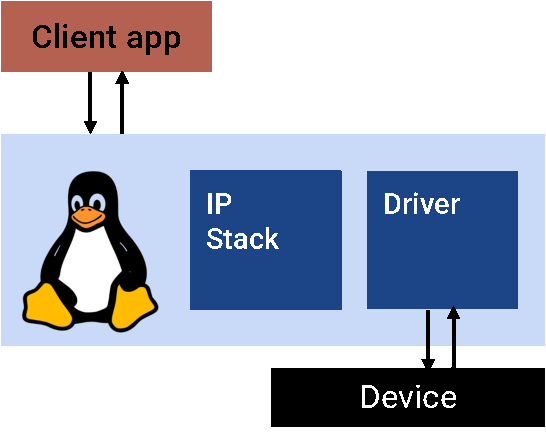
\includegraphics[width=6cm]{sockets.pdf}
	\caption{Network packet processing in a monolithic kernel.}
	\label{f:sockets}
\end{figure}

A monolithic operating system houses both drivers and protocol stacks in kernel as shown in
\autoref{f:sockets}. These components are typically written as libraries for the kernel to 
process a packet. In order for
a user application to utilise the network, the application must open a socket through a system
call. This system call creates an endpoint for communication and returns a file descriptor that refers
to that endpoint \cite{Linux:socket}. The file descriptor can then be used to read (receive a packet)
or write (transmit a packet) to the socket using the protocols specified when opening the socket.

To receive a packet on the network, the OS must first enqueue the addresses of buffers in memory to 
the device's control registers. The device can then write newly received data directly to these buffers. 
Once a packet has been written, the device will issue an interrupt to the OS to notify the OS. The 
kernel then processes this packet as defined by the IP protocol used in the packet. This typically 
includes reading the packet header, which contains critical information such as where the packet has
come from, where it is headed, as well as the communication protocol used. This information advises the
kernel about what to do with the packet. If the packet is addressed to a user-level application bound to
a socket, eventually the header of the packet will be stripped before the data is copied to a user space 
buffer queue attached to the socket. This buffer can now be accessed using a read (\emph{recv()}) system 
call. Note that much like a file read system call, this system call will block until there is data
available to be read.

To transmit, a user application can write a packet using a write (\emph{send()}) system call. 
The data will first be copied into an in kernel buffer. The kernel will process 
the packet and an appropriate header will be added to the head of the packet as per the protocol used 
with the socket. Eventually, this kernel buffer address will be enqueued to the device control
registers which signals to the device that a packet is ready for transmit, after which, the system call
returns. Once the device has transmitted the packet, it will issue an interrupt to notify the kernel
that the buffer is no longer in use and can be re-used.

Operating systems commonly use interrupt hold off on the device as an attempt to batch hardware
events, such as receiving or transmitting a packet, into a single interrupt. This means that the kernel
will be able to more efficiently process multiple packets at a time. At high throughputs on the receive
path, the kernel will even disable receive interrupts and switch to polling mode instead. This removes
the interrupt handling overhead but requires the driver to continuously check for hardware events.
Furthermore, in recent years, hardware has become more complex, and network devices are capable of 
commandeering some of the packet processing. This includes, for example, computing the packet
checksum or packet coalescing. Many of such hardware extensions have been capitalised on by monolithic
kernels to reduce the software overhead of packet processing.

%%%%%%%%%%%%%%%%%%%%%%%%%%%%%%%%%%%%%%%%%%%%%%%%%%%%%%%%%%%%%%%%%%%%%%%%%%%%%%%%%%%%%%%%%%%%%%%%%%%%%%%%%%%%%%%%%%%%%

However, the typical method of networking in a monolithic kernel is both insecure, due to the amount 
of untrusted code running at privilege level, and performs poorly, due to data copying operations and 
the increasing cost of system calls, particularly
those used for sending and receiving a packet \cite{Ren_RCVSY_19}.

\section{seL4}
\begin{figure}[h]
    \centering
    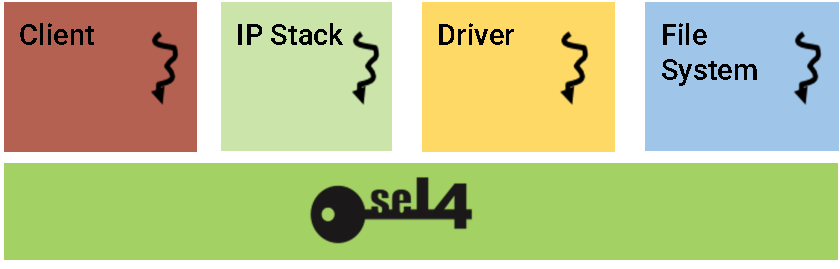
\includegraphics[width=8cm]{seL4.pdf}
    \caption{seL4 architecture}
    \label{f:sel4}
\end{figure}

seL4 is a highly performant, highly secure microkernel. It has been formally verified to be
functionally correct down to the binary, along with upholding the security properties confidentiality, 
integrity and availability \cite{Klein_AEMSKH_14}. However, as a microkernel, it provides only the minimum
to securely abstract the hardware and nothing more \cite{Heiser_PCVL_22}. As such, 
it presents a very low level API, and it does not provide resource management, file systems, network stacks
or device drivers and instead prescribes these services to run as user level programs. 
The kernel makes no distinction between such services and applications, which results in the horizontal
architecture shown in \autoref{f:sel4}. 

seL4 is also a capability based system. A capability is a communicable, unforgeable token that 
references a kernel object with an associated set of access rights. This provides fine grained access control
and means user-level components must have a capability in order to access an object and means that seL4
guarantees components only have access to objects, including data, that developers permit them to.
Additionally, seL4 guarantees ensure full isolation of user-level components, meaning that
failure of any component is completely contained and will not bring the rest of the system down. 
Finally, seL4 is the worlds fastest microkernel and performs within 25\%
of the limits imposed by hardware \cite{Mi_LYWC_19}. 

However, the microkernel design can potentially degrade performance as it requires
significantly more context switches than its monolithic counterpart. This is because OS services,
such as device drivers, typically run as an isolated components, and client
applications wishing to use such services must communicate using synchronous/asynchronous
IPC and shared memory. Furthermore, interrupt processing is forwarded to the user level handler
through asynchronous system calls and user level applications are also responsible for initiating
any cache management operations through system calls when required
for memory consistency. These system calls, which aren't typically required in a monolithic
system, can quickly add up. 

% Core Platform
\section{The seL4 Core Platform}
The seL4 Core Platform (seL4CP) is an operating system framework on seL4 with minimal abstractions over seL4 low level
objects \cite{Heiser_PCVL_22}. It aims to ease the development process of applications on seL4 by abstracting over
architecture specific details as well as seL4's low level API. seL4CP trades generality for simplicity and 
restricts systems to a predominantly static architecture. This means components are fixed at build time. 
The abstractions are:
\begin{enumerate}
    \item \textbf{Protection Domain (PD)}: a process abstraction that enforces an event driven programming model.
    \item \textbf{Communication Channel (CC)}: the ability for two PDs to communicate via notifications or PPCs.
    \item \textbf{Memory Region (MR)}: a range of physical memory that may be mapped into 1 or more PDs address spaces. 
    \item \textbf{Notification}: a semaphore-like synchronisation primitive. 
    \item \textbf{Protected Procedure Call (PPC)}: synchronous RPC between PDs. 
\end{enumerate}

seL4CP promotes the correct use of seL4 by employing an event driven driven programming model for PDs. Events are triggered by
either notifications or PPCs sent along a CC. seL4CP also restricts the use of seL4's IPC primitives to remote procedure calls,
which is only possible if the callee has strictly higher priority than the caller. This prevents PDs from either directly or 
indirectly calling themselves. Finally, while seL4CP predominantly only supports static systems, there is 
some supported dynamism which enables the re-initialising of PDs and dynamically loading code into PDs \cite{Heiser_PCVL_22}.
